\documentclass[twoside,11pt,a4paper]{article}

\usepackage[utf8]{inputenc}
\usepackage{amsmath, amssymb, latexsym}
\usepackage{sidecap}

\usepackage{tikz}
\usetikzlibrary{decorations.pathreplacing}

\begin{document}

\begin{SCfigure}[\sidecaptionrelwidth][t!]
	\centering
	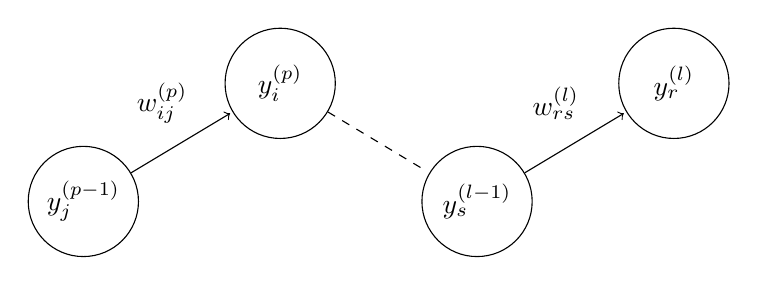
\begin{tikzpicture}[shorten >=1pt]
      		\tikzstyle{unit}=[draw,shape=circle,minimum size =1.4cm]

       	\node[unit](j) at (0,0){$y_j^{(p-1)}$};
        	\node[unit](i) at (2.5,1.5){$y_i^{(p)}$};

		\node[unit](s) at (5,0){$y_s^{(l-1)}$};
		\node[unit](r) at (7.5,1.5){$y_r^{(l)}$};
		
		\node at (1,1.25) {$w_{ij}^{(p)}$};
		\node at (6,1.25) {$w_{rs}^{(l)}$};
		
        	\draw[->] (j) -- (i);
        	\draw[dashed] (i) -- (s);
		\draw[->] (s) -- (r);
    	\end{tikzpicture}
	\caption[Exact evaluation of the Hessian.]{To derive an algorithm for evaluating the Hessian we consider two weights $w_{ij}^{(p)}$ and $w_{rs}^{(l)}$ where we assume that $p \leq l$. This figure illustrates the case when $p < (l - 1)$.}
	\label{fig:hessian}
\end{SCfigure}

\end{document}